\documentclass[12pt,a4paper,oneside]{report}

\usepackage[T1]{fontenc}
\usepackage{newtxtext}
\usepackage{xcolor}
\usepackage{graphicx}
\usepackage{lettrine}
\usepackage{forest}
\usepackage{tikz}
\usepackage{booktabs}
\usepackage{array}
\usepackage{float}
\usepackage{enumitem}
\usepackage{wasysym}
\usepackage{hyperref}

\hypersetup{
    colorlinks=true,
    linkcolor=blue,
    filecolor=magenta,      
    urlcolor=cyan,
    citecolor=blue,
    pdftitle={Your Document Title},
    pdfpagemode=FullScreen,
}

%--------------------------------------------------
% Lettrine settings
%--------------------------------------------------
\renewcommand*{\DefaultLoversize}{0.5}

%--------------------------------------------------
% Forest folder styling
%--------------------------------------------------
\definecolor{folderbg}{RGB}{124,166,198}
\definecolor{folderborder}{RGB}{110,144,169}

\def\Size{4pt}

\tikzset{
folder/.pic={
\filldraw[draw=folderborder,
top color=folderbg!50,
bottom color=folderbg]
(-1.05*\Size,0.2\Size+5pt)
rectangle ++(.75*\Size,-0.2*\Size-5pt);


\filldraw[draw=folderborder,
          top color=folderbg!50,
          bottom color=folderbg]
  (-1.15*\Size,-\Size)
  rectangle (1.15*\Size,\Size);


}
}

\begin{document}

\pagestyle{empty}

%--------------------------------------------------
% Title Page
%--------------------------------------------------
\begin{center}
	
\includegraphics[scale=0.7]{ialr-logo.png}


	\vspace{1.25cm}

	{\normalsize Coding and Robotics}\\[0.1cm]
	{\normalsize Applied Research Department}

	\vspace{1cm}

	{\Large\bfseries SMART Platform Imaging Software}\\[0.2cm]
	{\Large\bfseries Operations Manual}

	\vspace{0.75cm}
	
\end{center}

\cleardoublepage

%--------------------------------------------------
% Table of Contents
%--------------------------------------------------
\tableofcontents

\cleardoublepage

%--------------------------------------------------
% Introduction
%--------------------------------------------------
\chapter*{Introduction}
\addcontentsline{toc}{chapter}{Introduction}

\lettrine{T}{his} manual describes the installation and operation of the SMART Platform Imaging Software. The software is designed to process experimental imaging datasets generated by the SMART platform, and to consolidate the resulting data into structured Excel reports for visualization and group analysis.

The software consists of two primary modules:

\begin{itemize}
    \item \textbf{Analysis} --- Processes raw image folders into motion and size data, outputting per-plant Excel spreadsheets.
    \item \textbf{Data Consolidation} --- Merges all per-plant Excel files into a single workbook, with group assignment, chart generation, and optional plant filtering.
\end{itemize}

Before installation or operation, verify that the target computer satisfies the minimum hardware requirements outlined in Chapter~1.

\cleardoublepage

%--------------------------------------------------
% Chapter 1 - Hardware and Software
%--------------------------------------------------
\chapter{Hardware and Software}

This chapter describes the physical SMART platform hardware and the software used to process the imaging data it produces.

%%-------------------------------------------------
%% Section 1.1 - Hardware
%%-------------------------------------------------
\section{Hardware}

The SMART platform consists of a motorized X/Y gantry that positions a camera over each plant in turn for imaging. The primary hardware components are listed below:

\begin{itemize}
    \item \textbf{Three NEMA 17 stepper motors} --- Three 1.8$^\circ$ per step motors provide motion along the X, Y, and Z axes.
    \item \textbf{GRBL-based CNC controller} --- Controls all motion by interpreting G-code commands received over a serial connection.
    \item \textbf{Limit switches} --- Installed at the machine home position to establish the origin during the homing procedure.
    \item \textbf{24 V, 14.6 A power supply} --- Provides power to the motion control electronics and stepper motors.
    \item \textbf{USB camera} --- Mounted to the gantry for image acquisition at each plant location.
    \item \textbf{Light Strips} --- Approximately a minimum of 15 square feet of lighting laid across the top of the table to ensure lighting quality standard for imaging.
\end{itemize}

The GRBL controller communicates with the SMART Table Settings software over a serial connection at 115200 baud. During operation, the machine is first homed using the limit switches before executing the programmed imaging sequence. The camera captures an image at each predefined position as the gantry moves across the table.

\noindent\textbf{Note:} The limit switches are located only at the home (origin) position. No limit switches are installed at the maximum travel extents, so movements beyond the machine's physical limits are not automatically prevented once the machine has left the home position.
%%-------------------------------------------------
%% Section 1.2 - Software
%%-------------------------------------------------
\section{Software}

This section covers the SMART Platform Imaging Software: its system requirements, installation procedure, operation of the imaging table, and the data processing pipeline.

%%---------------------------------------
%% Subsection 1.2.1 - System Requirements
%%---------------------------------------
\subsection{System Requirements}

Before installing the SMART Platform Imaging Software, ensure that the computer meets the minimum hardware specifications listed below.

\begin{table}[h]
	\centering
	\begin{tabular}{>{\bfseries}l l}
		\toprule
		Requirement        & Minimum Specification \\
		\midrule           
		Processor          & 8 CPU cores or greater \\
		Available Memory   & 12 GB RAM or greater \\
		Free Storage Space & 10 GB minimum, or twice the size of the dataset being processed \\
		Operating System   & Windows 10 or Windows 11 \\
		\bottomrule
	\end{tabular}
\end{table}

\vspace{0.5cm}

The processor and memory specifications can be verified using the Windows \textit{System Information} utility.

\subsubsection*{Checking System Specifications}

\begin{enumerate}
	\item Press the \textbf{Windows} key.
	\item Type \textit{System Information}.
	\item Open the \textit{System Information} application.
	\item Select \textit{System Summary} from the navigation pane on the left.
\end{enumerate}

The navigation pane should appear similar to the example shown below.

\begin{center}
	\begin{forest}
		for tree={
				font=\ttfamily,
				grow'=0,
				child anchor=west,
				parent anchor=south,
				anchor=west,
				calign=first,
				inner xsep=7pt,
				edge path={
						\noexpand\path [draw,\forestoption{edge}]
						(!u.south west) +(7.5pt,0)
						|- (.child anchor)
						pic {folder}
						\forestoption{edge label};
					},
				before typesetting nodes={
						if n=1
							{insert before={[,phantom]}}
							{}
					},
				fit=band,
				before computing xy={l=15pt},
			}
			[System Summary
					[Hardware Resources]
					[Components]
					[Software Environment]
			]
	\end{forest}
\end{center}

The \textit{System Summary} page contains information similar to the table below.

\begin{table}[h]
	\centering
	\begin{tabular}{ll}
		\toprule
		Item                            & Value \\
		\midrule
		Processor                       & \dots \\
		Installed Physical Memory (RAM) & XX GB \\
		Total Physical Memory           & XX GB \\
		Available Physical Memory       & XX GB \\
		\bottomrule
	\end{tabular}
\end{table}

Verify that:

\begin{itemize}
	\item The processor contains at least \textbf{8 CPU cores}.
	\item The \textbf{Available Physical Memory} value is at least \textbf{12 GB}.
	\item The storage device used for processing has sufficient free space.
\end{itemize}

The recommended free storage capacity is either:

\begin{itemize}
	\item At least \textbf{10 GB}, or
	\item At least \textbf{twice the size} of the experimental dataset being processed,
\end{itemize}

whichever value is greater.

\vspace{0.5cm}

\noindent
\textcolor{red}{\textbf{WARNING:}}
If the minimum hardware requirements are not met, the software may become unresponsive or terminate unexpectedly during processing. This may result in loss of processed data and, in some cases, corruption of experimental datasets.

%%---------------------------------------
%% Subsection 1.2.2 - Installation
%%---------------------------------------
\subsection{Installation}

This section describes the installation procedure for the SMART Platform Imaging Software.

\vspace{1cm}

To download the software onto the target machine, proceed to the \href{https://github.com/mcostagliola-IALR/SMARTPlatformSoftware}{Github Repository}. Once on this page, download both the \textbf{mergeData} and \textbf{Analysis} folders. The installation directory is arbitrary, as long as the user has read and write permissions to the chosen location.

\vspace{0.5cm}

\noindent Once the folders have been downloaded, no further installation steps are required. The software can be launched directly from its folder.

\vspace{0.5cm}

\noindent You have now installed the SMART Platform Imaging Software onto your machine.

%%---------------------------------------
%% Subsection 1.2.3 - Table Operation
%%---------------------------------------
\subsection{Table Operation}

Physical operation of an imaging run --- moving the gantry over the table and capturing photos --- is controlled through a separate \textbf{SMART Table Settings} interface. This interface connects to the table's motion controller and camera, drives the gantry through a fixed imaging pattern, and captures a photo at each plant position.

\begin{figure}[H]
    \centering

    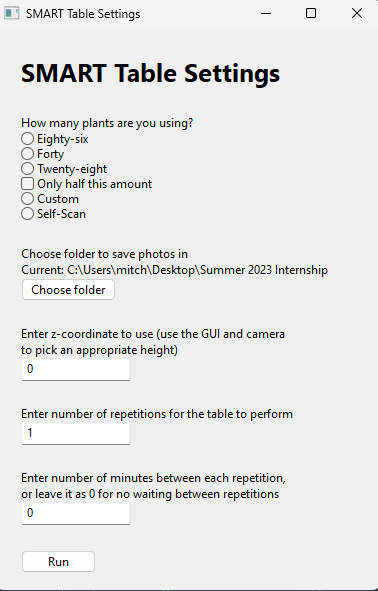
\includegraphics[width=0.5\textwidth]{img4.png}
    \caption{SMART Platform Control Software}
    \label{fig:third}
\end{figure}

\subsubsection*{Prerequisites}

Before running the table for the first time, a \texttt{config.txt} file must exist in the program folder containing three lines, in order:

\begin{enumerate}
    \item The destination folder where photos will be saved.
    \item The serial port name used by the table's controller (e.g.\ \texttt{COM3}).
    \item The numeric index of the USB camera to use.
\end{enumerate}

The destination folder can be changed at any time from within the interface (see below); the serial port and camera index must currently be set by editing \texttt{config.txt} directly.

\subsubsection*{Launching the Interface}

Run the SMART Table Settings program. A window titled \textbf{SMART Table Settings} will open, containing the controls described below.

\subsubsection*{Selecting a Layout}

Choose the imaging pattern to use, based on how the plants are arranged on the table:

\begin{itemize}
    \item \textbf{Eighty-six} --- 86-plant grid layout.
    \item \textbf{Forty} --- 40-plant grid layout.
    \item \textbf{Twenty-eight} --- 28-plant grid layout.
    \item \textbf{Custom} --- Uses a fixed list of coordinates read from \texttt{config.txt} instead of a built-in grid pattern.
    \item \textbf{Self-Scan} --- Automatically locates plants by detecting green pixels through the camera, then records their coordinates to \texttt{config.txt} for later use with Custom mode.
\end{itemize}

Check \textbf{Only half this amount} to image only half of the positions in the selected grid layout (43, 20, or 14 plants respectively). This option has no effect in Custom or Self-Scan mode.

\subsubsection*{Choosing a Photo Folder}

Click \textbf{Choose folder} to select the destination folder for captured images. The currently selected folder is shown above the button and is saved to \texttt{config.txt} automatically.

\subsubsection*{Setting Camera Height}

Enter a Z-coordinate in the height field to set the camera height used for every photo in the run. Determine an appropriate value beforehand using the table's positioning controls together with the camera preview. This is done in the config.txt file.

\subsubsection*{Repetitions and Interval}

\begin{itemize}
    \item \textbf{Repetitions} --- The number of times the table should image every plant, i.e.\ how many photos of each plant will be captured over the course of the run.
    \item \textbf{Interval} --- The number of minutes to leave between the start of each repetition. Leave at \textbf{0} to run repetitions back-to-back with no wait. If a repetition takes longer than the specified interval to complete, the next repetition begins immediately.
\end{itemize}

\subsubsection*{Running the Table}

Click \textbf{Run} to begin. The interface will:

\begin{enumerate}
    \item Connect to the table's motion controller over serial and initialize the camera.
    \item Home the machine.
    \item Move to each plant position in turn, capturing and saving a photo at each stop.
    \item Repeat the process for the configured number of repetitions, waiting between repetitions if an interval was set.
\end{enumerate}

Once \textbf{Run} is clicked, the settings window closes and progress messages are printed to the console, including an estimate of the total run time when an interval is set.

\vspace{0.5cm}

\noindent
\textcolor{red}{\textbf{WARNING:}}
Do not disconnect the camera or the controller, or interrupt power to the table, while a run is in progress. Doing so may leave the gantry in an unknown position and require re-homing before the table can be used again.

\vspace{0.5cm}

\noindent
\textcolor{red}{\textbf{NOTE:}}
The table's limit switches are located only at the home (origin) position. Movement commands that would drive the gantry out of bounds are not automatically caught away from home, so custom coordinates and camera heights should be verified carefully before an unattended run.

%%---------------------------------------
%% Subsection 1.2.4 - Data Processing
%%---------------------------------------
\subsection{Data Processing}

This section describes the data processing side of the SMART Platform Imaging Software. The software has two primary functions:

\begin{enumerate}
    \item \textbf{Analysis} --- Processes raw experimental image datasets and generates per-plant Excel reports containing motion, size, and supplementary data.
    \item \textbf{Data Consolidation} --- Merges the per-plant Excel reports produced by the Analysis function into a single unified workbook, with support for group assignment, chart generation, and selective plant filtering.
\end{enumerate}

\vspace{0.5cm}

Both functions are accessible from within the same application window via separate tabs at the top of the interface.

\begin{figure}[H]
    \centering

    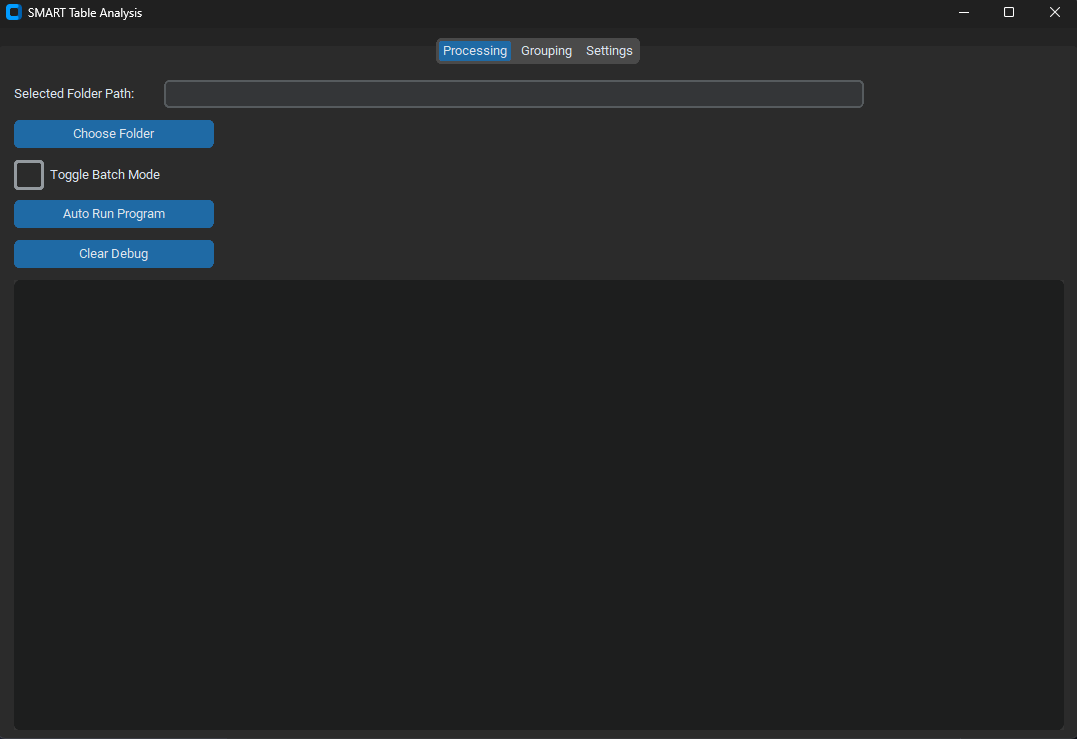
\includegraphics[width=\textwidth]{img1.png}
    \caption{Processing Tab}
    \label{fig:first}
\end{figure}

\begin{figure}[H]
    \centering

    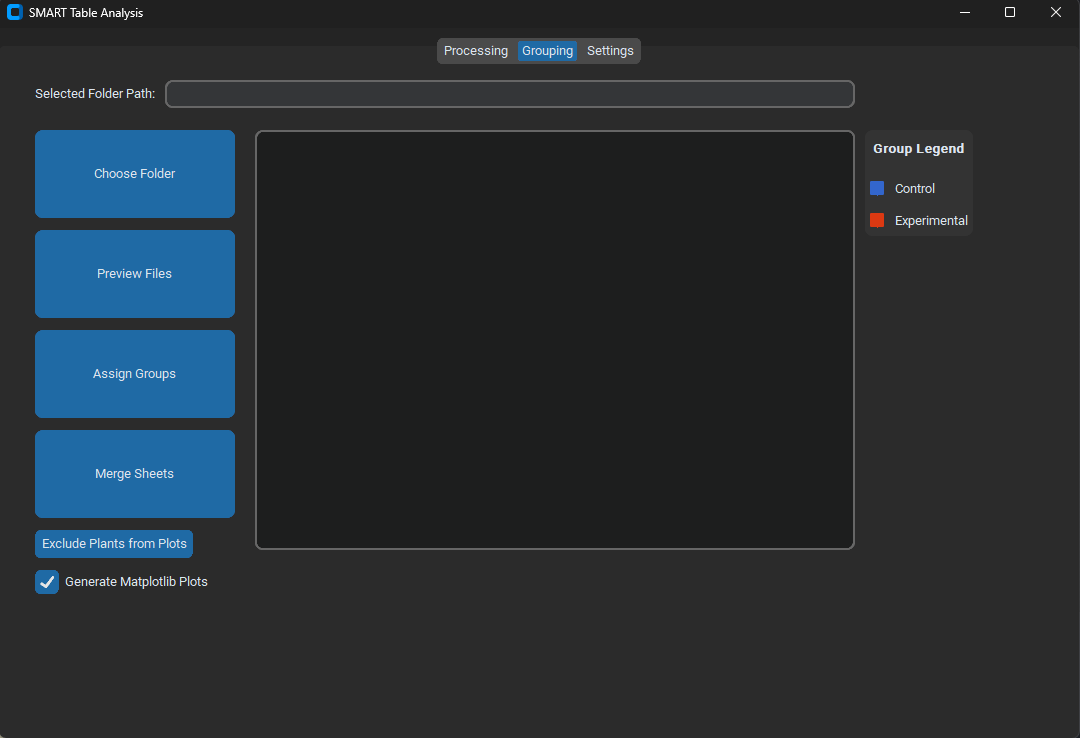
\includegraphics[width=\textwidth]{img2.png}
    \caption{Grouping Tab}
    \label{fig:second}
\end{figure}

\begin{figure}[H]
    \centering

    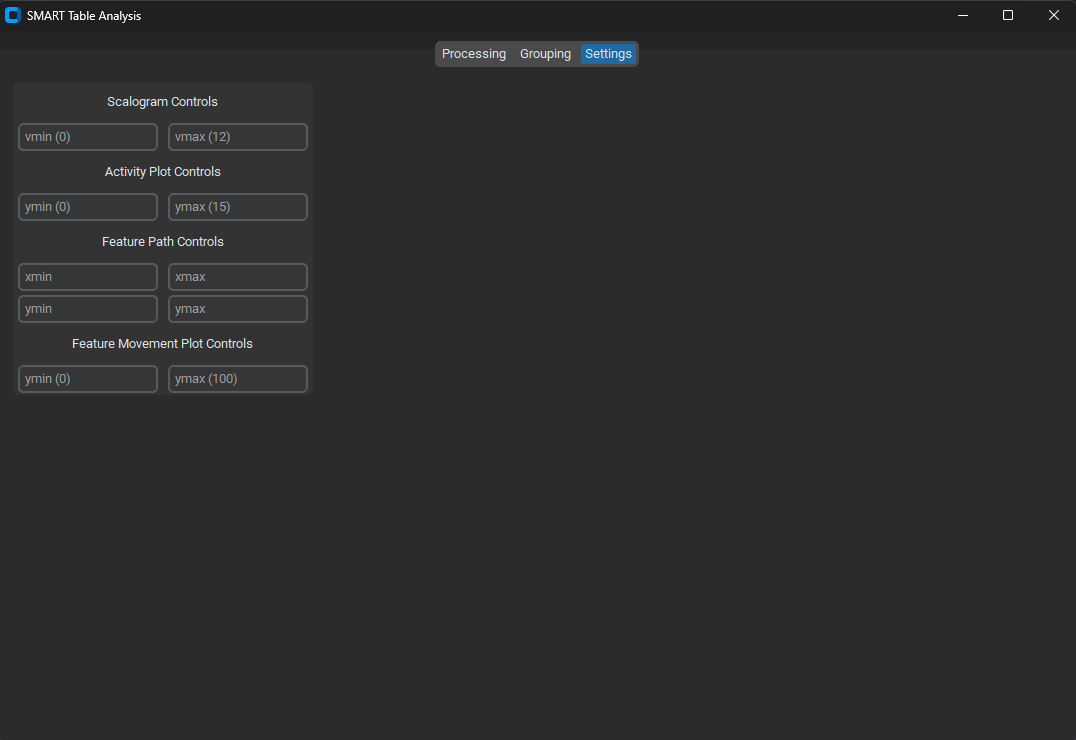
\includegraphics[width=\textwidth]{img3.png}
    \caption{Settings Tab}
    \label{fig:third}
\end{figure}

\subsubsection{Analysis}

The Analysis function processes datasets and generates an Excel spreadsheet containing movement, size, and other derived data for each plant. This spreadsheet will be saved within the folder that was selected for processing.

\paragraph{Processing Modes}

There are two processing modes available:

\begin{enumerate}
    \item \textbf{Single Folder Mode} --- Used to process a single plant folder, for example \texttt{Plant1}. Select the folder containing the raw image files directly.
    \item \textbf{Batch Processing Mode} --- Used to process an entire experiment at once. The selected folder should contain one subfolder per plant, following the topology shown below.
\end{enumerate}

\begin{center} 
\begin{forest}
for tree={
    font=\ttfamily,
    grow'=0,
    child anchor=west,
    parent anchor=south,
    anchor=west,
    calign=first,
    inner xsep=7pt,
    edge path={
        \noexpand\path [draw,\forestoption{edge}]
        (!u.south west) +(7.5pt,0)
        |- (.child anchor)
        pic {folder}
        \forestoption{edge label};
    },
    before typesetting nodes={
        if n=1
            {insert before={[,phantom]}}
            {}
    },
    fit=band,
    before computing xy={l=15pt},
}
[SL\_Tom\_11-8-24
    [Plant1]
    [Plant2]
    [Plant3]
    [...]
    [PlantX]
]
\end{forest}
\end{center}

\paragraph{Selecting a Processing Mode}

To select a processing mode, check or uncheck the \textbf{Toggle Batch Mode} checkbox in the Processing tab. When the checkbox is unchecked, the program operates in Single Folder Mode. When checked, the program operates in Batch Processing Mode. The button label updates to reflect the current mode.

\paragraph{Running the Analysis}

To run the Analysis function, follow the steps below:

\begin{enumerate}
    \item Select the desired processing mode using the \textbf{Toggle Batch Mode} checkbox.
    \item Click the \textbf{Choose File} or \textbf{Choose Folder} button and navigate to the target folder.
    \item Click \textbf{Auto Run Program} to begin processing.
\end{enumerate}

Progress and status messages will appear in the debug output window below the buttons. If an error occurs during processing, an error message will be displayed in the debug window along with the name of the file or folder that caused the issue.

\vspace{0.5cm}

\noindent
\textcolor{red}{\textbf{WARNING:}}
Do not close the application or navigate away from the Processing tab while the program is running. Doing so may interrupt processing and result in incomplete or missing output files.

\vspace{0.5cm}

When processing is complete, the output Excel file will be saved inside the processed plant folder. For batch mode, one Excel file will be generated per plant subfolder.

\subsubsection{Data Consolidation}

The Data Consolidation function is accessed from the \textbf{Grouping} tab. It collects all Excel files produced by the Analysis function from a selected folder, merges them into a single workbook, assigns plants to experimental groups, and generates charts for visualization.

\paragraph{Step 1: Select a Folder}

Click the \textbf{Choose Folder} button and navigate to the root directory of the experiment. This should be the same parent folder used during batch processing, containing all plant subfolders.

\paragraph{Step 2: Preview Files}

Click \textbf{Preview Files} to scan the selected folder for Excel files. The debug window will display a list of all detected files and the number of plants identified. This step must be completed before assigning groups or merging data.

\paragraph{Step 3: Assign Groups}

Click \textbf{Assign Groups} to open the group assignment window. Each detected plant will be listed alongside radio buttons corresponding to the available experimental groups.

\begin{itemize}
    \item By default, two groups are available: \textbf{Control} and \textbf{Experimental}.
    \item To add a new group, type a name into the text field at the bottom of the window and click \textbf{Add Group}.
    \item Select the appropriate group for each plant using the radio buttons.
    \item Click \textbf{Done} when all assignments are complete.
\end{itemize}

The group legend on the right side of the Grouping tab will update to reflect all current groups and their assigned colors.

\paragraph{Step 4: Exclude Plants from Plots (Optional)}

Click \textbf{Exclude Plants from Plots} to open the exclusion window. Plants are listed with checkboxes. Uncheck any plant to exclude it from the generated Matplotlib charts. Plants excluded here will still be included in the Excel output.

\paragraph{Step 5: Configure Chart Generation (Optional)}

Check or uncheck the \textbf{Generate Matplotlib Plots} checkbox to enable or disable the generation of \texttt{.png} chart files alongside the Excel output. This option is enabled by default.

\paragraph{Step 6: Merge Sheets}

Click \textbf{Merge Sheets} to begin the consolidation process. The program will:

\begin{enumerate}
    \item Read all detected motion and size Excel files.
    \item Merge the data into a single workbook with two worksheets: \texttt{Motion\_Worksheet} and \texttt{Size\_Worksheet}.
    \item Generate embedded Excel charts for both motion and size data, color-coded by group.
    \item Optionally generate external \texttt{.png} chart files (\texttt{motion\_chart.png} and \texttt{size\_chart.png}).
    \item Save the output as \texttt{Merged.xlsx} in the selected folder.
\end{enumerate}

A confirmation dialog will appear when the file has been created successfully. If \texttt{Merged.xlsx} already exists in the selected folder, the program will prompt you to confirm before overwriting it.

\vspace{0.5cm}

\noindent
\textcolor{red}{\textbf{WARNING:}}
Do not modify or open any of the source Excel files while the merge is in progress. This may cause file access errors and prevent the output from being generated.

\subsubsection{Settings}
\label{sec:settings}

The \textbf{Settings} tab provides controls for adjusting the axis limits of the plots generated during the Analysis phase. The available controls are listed below.

\begin{table}[H]
    \centering
    \begin{tabular}{>{\bfseries}l l}
        \toprule
        Control & Description \\
        \midrule
        Scalogram vmin / vmax & Minimum and maximum color scale values for scalogram plots \\
        Activity Plot ymin / ymax & Y-axis bounds for activity line plots \\
        Feature Path xmin / xmax & X-axis bounds for feature path plots \\
        Feature Path ymin / ymax & Y-axis bounds for feature path plots \\
        Feature Movement ymin / ymax & Y-axis bounds for feature movement plots \\
        \bottomrule
    \end{tabular}
\end{table}

Leave any field blank to use the default value shown in the placeholder text. Settings are applied the next time \textbf{Auto Run Program} is executed.

\cleardoublepage

%--------------------------------------------------
% Chapter 2 - Output Files
%--------------------------------------------------
\chapter{Output Files}

This chapter describes the files generated by the software and their locations.

\section*{Analysis Output}

For each processed plant folder, the following files are generated inside that folder:

\begin{table}[H]
    \centering
    \begin{tabular}{>{\ttfamily}l p{9cm}}
        \toprule
        \normalfont\textbf{File} & \textbf{Description} \\
        \midrule
        motion\_analysis\_report.xlsx & Contains per-frame displacement data for the plant on the \texttt{Displacement Data} sheet. \\
        mask\_sizes.xlsx & Contains per-frame pixel count data for the plant on \texttt{Sheet1}. \\
        \bottomrule
    \end{tabular}
\end{table}

\section*{Data Consolidation Output}

The following files are generated inside the root experiment folder after running \textbf{Merge Sheets}:

\begin{table}[H]
    \centering
    \begin{tabular}{>{\ttfamily}l p{9cm}}
        \toprule
        \normalfont\textbf{File} & \textbf{Description} \\
        \midrule
        Merged.xlsx & Consolidated workbook containing motion and size data for all plants, with embedded Excel charts color-coded by group. \\
        motion\_chart.png & Matplotlib chart of plant displacement over time (generated if the plot option is enabled). \\
        size\_chart.png & Matplotlib chart of plant pixel count over time (generated if the plot option is enabled). \\
        \bottomrule
    \end{tabular}
\end{table}

\cleardoublepage

%--------------------------------------------------
% Chapter 3 - Experiment Setup Recommendations
%--------------------------------------------------
\chapter{Experiment Setup Recommendations}

\lettrine{T}{he} SMART Platform Imaging Software relies on color-based image segmentation to isolate plants from their surroundings. The accuracy of this segmentation — and therefore the reliability of all motion and size data — is directly determined by the physical setup of the experiment. This chapter describes the conditions under which segmentation performs best, and the setup choices that should be avoided.

\vspace{0.5cm}
The Platform should be in a air controlled environment. The electronics will give off heat sufficient to raise the ambient air temperature depending on the size of the room.

\vspace{0.5cm}

\noindent
\textcolor{red}{\textbf{NOTE:}} The segmentation algorithm is designed for \textbf{majority-green plants}. Species or growth stages where the plant is predominantly yellow, brown, purple, or white are not reliably segmented and may produce inaccurate size measurements.

%%-------------------------------------------------
%% Section 3.1 - Background
%%-------------------------------------------------
\section{Background}

The single most important factor in segmentation quality is the contrast between the plant and its background. The software identifies plant pixels by detecting green hues that stand out from the surrounding area. If the background contains similar colors or textures, the segmentation boundary becomes ambiguous.

\subsection*{Recommended}

\begin{itemize}
    \item Use a \textbf{uniform dark background} — matte black fabric, black felt, or black grow bags produce the highest contrast against green plant tissue and are strongly preferred.
    \item Ensure the background material is \textbf{non-reflective}. Shiny or glossy surfaces can produce specular highlights that the algorithm may misclassify as plant tissue.
    \item The background should be \textbf{consistent across all images} in an experiment. Changes in background material between imaging sessions will introduce inconsistencies in the size measurements over time.
\end{itemize}

\subsection*{Avoid}

\begin{itemize}
    \item \textbf{Brown or tan substrates} such as exposed soil, coco coir, or peat visible in frame. These materials contain warm color tones that partially overlap with plant hue values and will be incorrectly included in the mask.
    \item \textbf{Green or blue-green containers}, trays, or pots. Any container color in the green hue range will be detected as plant material.
    \item \textbf{Patterned or textured backdrops} such as woven fabric with a visible weave pattern. Fine texture can produce noise at the segmentation boundary.
\end{itemize}

%%-------------------------------------------------
%% Section 3.2 - Substrate Visibility
%%-------------------------------------------------
\section{Substrate and Container Visibility}

The growing substrate — soil, perlite, coco coir, rockwool, or similar media — should not be visible in the image frame. Even small exposed areas of substrate around the base of the plant can produce false positives in the mask, inflating the reported plant size.

\subsection*{Recommended}

\begin{itemize}
    \item \textbf{Cover exposed substrate} around the plant base with black fabric, black landscape cloth, or a fitted cover cut to the container opening. This eliminates the substrate from the camera's field of view entirely.
    \item Position the camera so that the \textbf{container rim is not visible}, or ensure it is a dark neutral color that does not fall within the green hue detection range.
    \item If using net pots or open containers, \textbf{wrap or cover the pot exterior} with black material before imaging.
\end{itemize}

\subsection*{Avoid}

\begin{itemize}
    \item Leaving \textbf{bare substrate exposed} around the plant stem. This is the most common source of segmentation error in practice.
    \item Using \textbf{white or light-colored grow media} such as perlite or hydroton without covering, as these reflect light and create bright regions the algorithm was not designed to exclude.
    \item \textbf{Wet substrate surfaces}, which can produce dark reflective patches that interfere with the background detection step.
\end{itemize}

%%-------------------------------------------------
%% Section 3.3 - Lighting
%%-------------------------------------------------
\section{Lighting}

The segmentation algorithm performs best when the plant is \textbf{evenly and adequately illuminated}. The example images shown in this manual were captured under relatively low ambient light, which required the algorithm to perform additional brightness correction before segmentation. While the software handles underexposed images, consistent and diffuse lighting reduces processing error and improves measurement repeatability.

\subsection*{Recommended}

\begin{itemize}
    \item Use \textbf{diffuse, even illumination} across the plant canopy. Softbox lighting or LED grow panels with a wide beam angle reduce hard shadows between leaves.
    \item Ensure lighting is \textbf{consistent between imaging sessions}. Changes in light intensity or angle over the course of an experiment will cause apparent changes in plant size that are artefactual rather than biological.
    \item If imaging under natural or greenhouse light, \textbf{image at the same time of day} for every session to minimize variation in sun angle and intensity.
\end{itemize}

\subsection*{Avoid}

\begin{itemize}
    \item \textbf{Hard directional lighting} that casts strong leaf shadows onto the background or onto other leaves. Shadow regions on the plant can fall below the detection threshold and appear as holes in the mask.
    \item \textbf{Backlighting} or light sources positioned behind the plant relative to the camera, which reduces apparent leaf contrast.
    \item \textbf{Mixed color temperature light sources} in the same frame, for example a cool white grow light combined with warm incandescent ambient light, which shifts hue values unpredictably.
\end{itemize}

%%-------------------------------------------------
%% Section 3.4 - Plant Suitability
%%-------------------------------------------------
\section{Plant Suitability}

The segmentation algorithm detects plant pixels by identifying green hues within a defined range. Plants that fall outside this range at any point during the experiment will not be accurately segmented.

\subsection*{Compatible Plant Types}

\begin{itemize}
    \item Plants with \textbf{predominantly green foliage} throughout the experimental period.
    \item Species with \textbf{flat or broad leaves} viewed from above produce the cleanest masks, as leaf area is maximally exposed to the camera.
    \item Plants at \textbf{vegetative growth stages} where green leaf tissue dominates the canopy.
\end{itemize}

\subsection*{Incompatible or Problematic Cases}

\begin{itemize}
    \item \textbf{Severely stressed or senescing plants} where significant yellowing, browning, or necrosis has occurred. Yellow tissue falls outside the green hue detection range and will be excluded from the mask, underreporting true plant size.
    \item \textbf{Purple or anthocyanin-rich varieties} such as red lettuce or purple basil. These cultivars contain little green pigment and will produce very small or empty masks.
    \item \textbf{Seedlings at germination stage} where only the hypocotyl and cotyledons are visible. These structures are very small and may fall below the minimum area threshold used to filter noise. The fill threshold parameter described in the Settings subsection of the Hardware and Software chapter (Section~\ref{sec:settings}) may need to be reduced for early-stage imaging.
    \item Plants where \textbf{flowers, fruit, or senescent tissue} constitute a large fraction of the visible canopy, as these structures are typically non-green and will be excluded from the size measurement.
\end{itemize}

%%-------------------------------------------------
%% Section 3.5 - Summary Checklist
%%-------------------------------------------------
\section{Pre-Experiment Setup Checklist}

Before beginning an imaging experiment, verify each of the following conditions:

\begin{itemize}
    \item[\Square] Background is dark, matte, and uniform across all imaging positions.
    \item[\Square] All exposed substrate around the plant base is covered with black material.
    \item[\Square] Container exteriors are dark or covered and do not fall within the green hue range.
    \item[\Square] Lighting is diffuse, even, and will remain consistent across all imaging sessions.
    \item[\Square] Plant species is majority-green and at a vegetative growth stage.
    \item[\Square] Camera position is fixed and will not shift between imaging sessions.
    \item[\Square] A test image has been processed through the Analysis function and the resulting mask reviewed before committing to a full experiment run.
\end{itemize}

\cleardoublepage

%--------------------------------------------------
% Chapter 4 - Troubleshooting
%--------------------------------------------------
\chapter{Troubleshooting}

\begin{table}[H]
    \centering
    \begin{tabular}{p{5.5cm} p{8cm}}
        \toprule
        \textbf{Problem} & \textbf{Resolution} \\
        \midrule
        No Excel files found during preview & Verify that the correct root folder has been selected and that the Analysis step has been completed for at least one plant. \\
        \addlinespace
        Error processing a specific file & Check that  the file is not open in another application. Ensure the file was generated correctly by the Analysis function and has not been manually modified. \\
        \addlinespace
        Merged.xlsx is missing charts & Ensure that plant groups have been assigned before clicking Merge Sheets. If groups are unassigned, all plants default to the Control group color. \\
        \addlinespace
        Matplotlib charts are not generated & Verify that the \textbf{Generate Matplotlib Plots} checkbox is enabled and that at least one plant is not excluded in the Exclude Plants window. \\
        \addlinespace
        Software becomes unresponsive during processing & This may indicate insufficient system memory. Verify that available RAM meets the minimum requirement of 12~GB and close other applications before restarting the software. \\
        \addlinespace
        Debug window shows output from the wrong tab & Switch to the desired tab before running any operation. The debug output window updates to the active tab automatically. \\
        \bottomrule
    \end{tabular}
\end{table}

\chapter{Future Considerations}

The SMART Platform Imaging Software has been designed to provide an extensible platform for automated plant imaging and data analysis. Future development may include improvements in both the hardware and software to increase functionality, usability, and processing efficiency.

\section{Hardware}

Potential hardware enhancements include:

\begin{itemize}
    \item Installation of limit switches at the maximum travel extents to provide additional protection against out-of-bounds movement.
    \item Integration of improved lighting systems to provide more consistent image quality across experiments.
    \item Support for higher-resolution or industrial machine vision cameras.
    \item Light absorbing background or increased layering of landscape fabric to decrease luminence in images.
\end{itemize}

\section{Software}

Potential software enhancements include:

\begin{itemize}
    \item Automatic software update functionality.
    \item Support for additional image analysis algorithms and plant phenotyping metrics.
    \item GPU acceleration to reduce processing time for large datasets.
    \item Automatic detection of hardware devices, eliminating manual configuration of serial ports and camera indices.
    \item Expanded data visualization and statistical analysis tools.
    \item Additional export formats for processed data and reports.
    \item Cross-platform compatibility with Linux and macOS.
    \item Support for various varieties of various color ranges --- not just primarily green varieties.
\end{itemize}

The modular design of both the SMART platform hardware and the SMART Platform Imaging Software allows new capabilities to be incorporated with minimal changes to the overall workflow.

\end{document}